\chapter{Evolution of System User Interactive Tests}
\section{Introduction}
\label{sec:evolution-introduction}

This section presents Keyword-Driven Testing (KDT) , along with illustrative examples and a description of its supporting framework, Robot Framework \cite{RobotFramework2020}, and the industrial context of our study.

\subsection{Keyword-Driven Testing}
\label{kdt}

Keyword-Driven testing (KDT) is a software testing technique that aims at separating test design from the technical implementation of the tests, thus, limiting exposure to unnecessary details and avoiding duplication. KDT advocates that this separation of concerns allows tests to be written easier, to create more maintainable tests and enables experts from different fields and backgrounds to work together, at different levels of abstraction, for the creation of the tests.

To do so, KDT\cite{Tang2008} aims at separating test design from technical implementation. Its goal is to limit the exposure to unnecessary details and avoiding duplication. KDT advocates that this separation of concerns allows tests to be written easier, to create more maintainable tests and enables experts from different fields and backgrounds, work together at different levels of abstraction. 

Figure~\ref{fig:robotframework_script} shows an example of a KDT test. This test, named ``Valid Login'' (line 5, adopted from the official documentation of Robot Framework), is responsible for validating the correct behaviour of the login form in an imaginary SUT. Lines 6--8 present the ``steps'' of the tests and, in KDT parlance, they are calls to \emph{keywords}. In turn, these keywords are defined in the respective definition blocks between lines 10 and 28. Each keyword is itself decomposed in a series of steps. Keywords can have \emph{arguments}. For instance, keyword ``Open browser'' (line 12) takes two arguments, ``\$\{LOGIN URL\}'' and ``\$\{BROWSER\}''. The use of arguments to call keywords allows to further extend the reuse of keywords.

As can be seen from the figure, most part of this fully automated test is written in plain English. This enables the unobstructed collaboration in the creation of the tests between different experts. For instance, a business analyst can write the high-level part of the test (lines 4--8) and an automation expert can implement the remaining part of the test (lines 10-35), adding the technical details to automate the steps.

\begin{figure}[t!]
\centering
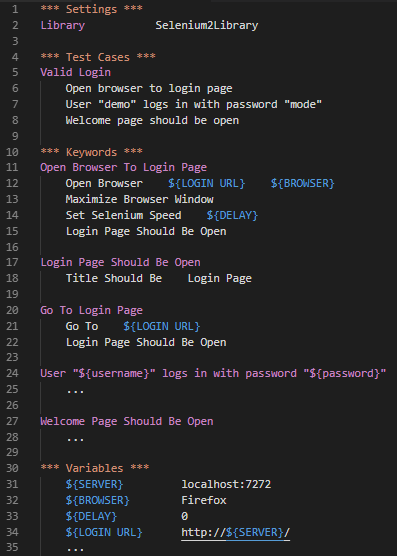
\includegraphics[width=\columnwidth]{figures/evolution/robotframework_script.png}
\caption{An example of a KDT test.}
\label{fig:robotframework_script}
\end{figure}

% \footnotetext{Some of the keywords were omitted for visibility constraints}

KDT tests can be represented using a tree structure. Figure~\ref{fig:robotframework_tree} shows this structure for the test of Figure~\ref{fig:robotframework_script}. The root of the tree (purple rectangle) is the \emph{Test Case} that is executed by calling all the keywords contained. The intermediary nodes (white rectangles) are called \emph{User Keywords} since they are created by the tester. Finally, the leaf nodes (green rectangles) are \emph{Library Keywords}. \emph{Library Keywords} are implemented by the system or an external library and responsible for either controlling the control flow of the tests or interacting with the SUT.

\begin{figure}[t!]
\centering
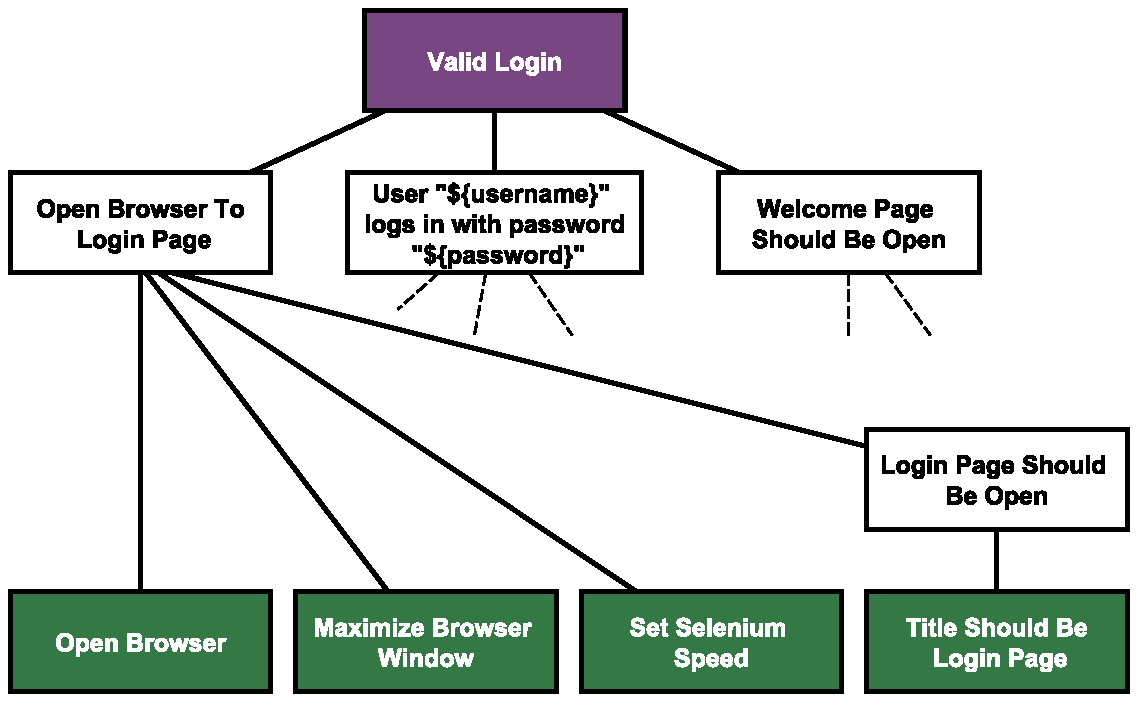
\includegraphics[width=\columnwidth]{figures/evolution/robotframework_tree.pdf}
\caption{Tree representation of the ``Valid Login'' KDT test.}
\label{fig:robotframework_tree}
\end{figure}

We group keywords into seven categories based on their functionality and present them in Table \ref{keywords_categories}. We define a \emph{SYNC}
keyword category for keywords dealing with the synchronization between tests and SUT; e.g., a keyword that waits 10 seconds for a GUI element of the SUT to become available. In the rest of the paper we use the term keyword to refer to \emph{User Keywords} unless stated otherwise.

\subsection{Robot Framework}
\label{robot_framework}

One the tools used for the application of KDT is Robot Framework \cite{RobotFramework2020}. Robot Framework is a popular framework used world-wide by major companies, including Nokia, KONE, ABB. This is also the tool adopted by our industrial partner and, thus, used in this work. Robot Framework is an open source tool originally developed by Nokia Networks and is mainly used for acceptance testing. The ``Valid Login'' KDT test of Figure \ref{fig:robotframework_script} was written using this framework.

One of the main advantages of Robot Framework is its high modularity.  Indeed, Robot Framework is platform-agnostic and thanks to its driver plugin architecture, the core framework does not require any knowledge of the SUT. For instance, in Figure~\ref{fig:robotframework_script}, lines 1--2 show that the script is using the external library for Selenium to interact with the SUT. Another advantage of the framework lies in its simple syntax, which makes it easily accessible to testers, regardless of their background.

\begin{table}
\caption{Keyword categories}
\label{keywords_categories}
\centering
\begin{tabular}{>{\raggedright}m{0.9in}>{\raggedright}m{2.3in}}
\toprule
\textbf{\scriptsize{Label}} & \textbf{\scriptsize{Explanation}}\tabularnewline
\toprule

\scriptsize{\textit{ACTION}}    & \scriptsize{Keyword performing an action on the
SUT capable of modifying its state.} \tabularnewline

\scriptsize{\textit{ASSERTION}} & \scriptsize{Keyword verifying that a predicate
is true at a specific point of test execution} \tabularnewline

\scriptsize{CONTROLFOW}         & \scriptsize{Keyword allowing to modify the
                                   control flow of the test execution.} \tabularnewline

\scriptsize{GETTER}             & \scriptsize{Keyword allowing to extract an element from
the SUT.} \tabularnewline

\scriptsize{LOGGING}            & \scriptsize{Keyword dumping logs during execution.}
\tabularnewline

\scriptsize{SYNC}               & \scriptsize{Keyword relating to the
                                  synchronization between the SUT and the tests.} \tabularnewline

\scriptsize{\textit{USER}}      & \scriptsize{Keyword created by a user.}
\tabularnewline

\bottomrule
\end{tabular}
\end{table} 

\subsection{Industrial Context}
\label{sec:evolution-introduction-data}

In this work, we aim at investigating the evolution of KDT test suites at the acceptance testing level based on the industrial practice. To this end, we work together with BGL BNP Paribas that has recently (1 year ago) adopted KDT and uses it in its daily software development work for acceptance testing.

One of the reasons that our partner adopted KDT is that test cases at this testing level were created by different domain experts (business analysts and automation experts) and the adoption of a common language between the experts was imperative. All the tests used in our study have been created by a team of 3 testers and 2 business analysts working at BGL BNP Paribas using Robot Framework.

The project used in our study, hereafter referred to as \emph{SubjectA} for confidentiality reasons, pertains to all the business activities of our partner. The front-end is a web application implemented in AngularJS, and, the back-end is composed of hundreds of services written in various programming languages. These services are managed by different teams, involving more than 100 developers. The KDT test suite used in our study, referred to as \emph{TestSuiteA}, is developed by 3 testers working at the Quality Assurance (QA) team of our partner and 2 business analysts.

\begin{figure}[t!]
  \centering
  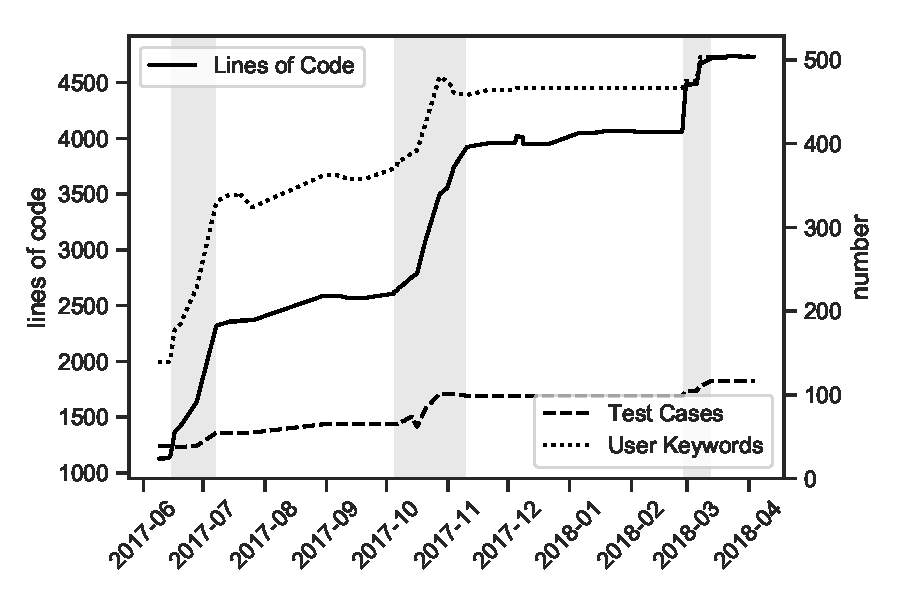
\includegraphics[width=0.7\columnwidth]{figures/evolution/project_evolution.pdf}
  \caption{Evolution of TestSuiteA}
  \label{fig:project_evolution}%\setlength{\tabcolsep}{5.1px} 
\end{figure}

Figure~\ref{fig:project_evolution} shows the evolution of TestSuiteA across the eight-month period studied. The figure depicts the evolution of the number of \emph{Test Cases} comprising the test suite, the number of \emph{User Keywords} and the lines of code of the test suite. As can be seen, our analysis begins with a test suite of 39 test cases, 139 user keywords and 1129 lines of code and ends with 117 test cases, 505 keywords and 4732 lines of code.

In the time span depicted in Figure~\ref{fig:project_evolution}, we isolated three periods during which we saw an increased test creation activity (shown in grey). After discussing with the QA team, they corroborated that these periods were more focused on test creation and the remaining ones on test maintenance. Thus, we analyze separately these periods (greyed and non-greyed) and refer to them as ``Creation'' and ``Maintenance''.

\section{Research Questions}

In this study, we attempt to answer two main questions about KDT test suites at the acceptance testing level: ``\emph{What are the benefits and challenges of adopting KDT?}''  and ``\emph{What kind of changes are performed during the evolution of a KDT test suite?}''. Answers to these questions will enable practitioners to make more informed decisions about KDT and will improve our understanding of KDT test suite evolution. Thus, we pose the following research questions:

\begin{description}
\item[\textbf{RQ1}:] \emph{What types of test code changes are performed during KDT test suite evolution?}
\end{description}

Analyzing the changes performed by the testers during KDT test suite evolution forms the basis of any automated test refactoring and test repair technique. Although research presents such information in the case of unit testing \cite{Pinto2012}, no previous study has discussed such fine-grained changes in the context of KDT at the acceptance level, to the best of our
knowledge.

\begin{description}
\item[\textbf{RQ2}:] \emph{How complex are the KDT test suites and how does this complexity affect their evolution?}
\end{description}

As mentioned in Section \ref{sec:evolution-introduction}, one of the advantages of KDT is that it allows the separation of the technical implementation details of test code and its corresponding intention. This fact can lead to test suites having several ``levels of abstraction'' (cf. Figure \ref{fig:robotframework_tree}). To this day, it is not clear how complex the KDT test code is and how this complexity affects its evolution. Answering this question will provide us with a better understanding of the difficulties faced by practitioners when they try to apply KDT and can guide future research directions in ameliorating these problems.

\begin{description}
\item[\textbf{RQ3}:] \emph{Does code duplication exist in KDT test code bases? What is its impact on the evolution of the test code?}
\end{description}

Similar code fragments are known to exist in source code and test code alike \cite{Baker1995, Roy2009, Rattan2013, Lavoie2017}. In RQ3, we investigate whether KDT codebases contain duplicated test code and how these test clones affect the evolution of the test codebase. Answering this research question is important because if such test clones exist, we need to investigate appropriate techniques to detect them, analyze them and monitor their evolution.

\begin{description}
\item[\textbf{RQ4}:] \emph{What are the practitioners' perceptions of the
    benefits and challenges of KDT in practice?}
\end{description}

RQ4 pertains to documenting and analyzing the practitioners' opinion about the advantages and disadvantages of KDT. Such analysis can help other testers to adopt (or not) KDT. Additionally, this research question gives us the opportunity to ask the practitioners' opinion about our results, validating them and understanding them better.

\section{Research Protocol}

\subsection{Definitions}
\label{sec:evolution-protocol-definitions}

\begin{itemize}
    \item \textbf{Tree}: Keywords can be represented as trees, thus, we can define a $tree\; T$ as an ordered, directed, acyclic graph with nodes $N(T)$ and edges $E(T) \subseteq N(T) \times N(T)$. The nodes of the tree denote keywords and each edge between two keywords denotes a ``step'': the parent keyword has the child keyword as a \emph{step}. For instance, in Figure \ref{fig:robotframework_tree}, keyword ``Open Browser To Login Page'' has four steps: ``Open Browser'', ``Maximize Browser Window'', ``Set Selenium Speed'' and ``Login Page Should Be Open''. As the tree is ordered, the execution of the steps will follow the order in the tree, from left to right. A node with no parent is a $root$ node that should be defined in the \emph{Test Case} block,  while a node with no children is a $leaf$ node and should be a \emph{Library Keyword}.

    \item \textbf{Keyword Level}: The \emph{level} of keyword $k$, is the maximum number of edges that exist on the subpath(s) from $k$ to a leaf keyword. In Figure \ref{fig:robotframework_tree}, ``Login Page Should Be Open'' is a \emph{level 1} keyword whereas ``Open Browser To Login Page'' is a \emph{level 2}. \emph{Library Keywords} at the leaves of the tree have a \emph{level 0}.

    \item \textbf{Keyword Connectivity}: Connectivity is a metric of reusability among the keywords. A keyword can belong to several test cases represented as trees: let keyword $k$ belong to trees $T_1, T_2, ... T_n$, i.e. $k \in N(T_1) \cup N(T_2) \cup ... \cup N(T_n)$, then we calculate the connectivity of $k$ by counting the number of nodes (keywords) in the subpath(s) from the root nodes of $T_1, T_2, ... T_n$ to $k$.

    \item \textbf{Keyword Churn}: Keyword churn is the number of lines of code added, edited or deleted from one version to the next over a period of time.
\end{itemize}

The last 3 definitions correspond to metrics used in our study. The \emph{keyword level} is used to group keywords having equal levels together. According to the philosophy of KDT, lower level keywords should be more linked to the technical details of the SUT whereas higher level keywords should be more abstract, expressing the functional requirements. The \emph{ connectivity} metric expresses the degree to which a keyword is reused and, as a consequence, the degree to which a change to this keyword can impact the test suite. Finally, the \emph{churn} corresponds to the degree to which a keyword is changed during the evolution of the test suite.

\subsection{Answering RQ1}
\label{sec:evolution-protocol-rq1}

To answer RQ1, we extract all the changes occurring in the test suite and group them per type of change. The types identified describe an action (insert, update, delete) performed on a code unit element (\emph{User Keyword}, \emph{Test Case}, \emph{Variable}, etc.). 

To this end, we extracted the 129 commits from the evolution of TestSuiteA. For each pair of consecutive commits, we gather the changes using a fine grain change algorithm.

The algorithm relies on previous, state-of-the-art studies \cite{Chawathe1996, Falleri2014, Fluri2007, Pinto2012}. In these studies, the authors built abstract syntax trees (ASTs) of Java classes and used tree edit distance algorithms to extract an optimal change path from one tree to the other, with each tree corresponding to a version of the code base.

To detect the changes, the algorithm works in two phases:

\begin{enumerate}
    \item Finding a match between elements of $v_1 \in V$ and $v_2 \in V$ where $V$ is the set of versions -- with one version corresponding to one commit -- to come up with a mapping $e_{1n} \rightarrow e_{2n}$ where $e_{mn} \in E_n$ and $E_n$ is the set of elements from $v_n$.
  
    \item Finding a minimum edit script that transforms $V_1$ to $V_2$ given the computed mapping.
\end{enumerate}

Phase 1 is essential to the edit script since the more elements that can be matched, the better the minimum edit script will perform. Phase 2 produces  an edit script detecting the basic edit operations \emph{INSERT}, \emph{UPDATE}, \emph{DELETE} for each pair of matched elements.

\begin{algorithm}[!t]
\caption{Element Matcher}
\label{alg:element_matcher}
\begin{algorithmic}[1] 
\REQUIRE $E_1 \subset v_n$, $E_2 \subset v_{n+1}$
\ENSURE final matching set: $M_{final}$
\STATE $M_{final} \leftarrow \emptyset$
\STATE $E_{1,unmatched} \leftarrow \emptyset$
\FOR{$e_1 \in E_1$}
\IF{$findMatchFileAndName(e_1,E_2)$}
\STATE $M_{final} \leftarrow M_{final} \cup (e_1,e_2)$
\STATE $E_2 \leftarrow E_2 - e_2$
\ELSE
\STATE $E_{1,unmatched} \leftarrow E_{1,unmatched} \cup e_1$
\ENDIF
\ENDFOR
\FOR{$e_1 \in E_{1,unmatched}$}
\IF{$findMatchFileAndContent(e_1,E_2)$}
\STATE $M_{final} \leftarrow M_{final} \cup (e_1,e_2)$
\STATE $E_2 \leftarrow E_2 - e_2$
\ELSIF{$findMatchNameAndContent(e_1,E_2)$}
\STATE $M_{final} \leftarrow M_{final} \cup (e_1,e_2)$
\STATE $E_2 \leftarrow E_2 - e_2$
\ELSE
\STATE $M_{final} \leftarrow M_{final} \cup (e_1,\emptyset)$
\ENDIF
\ENDFOR
\FOR{$e_2 \in E_2$}
\STATE $M_{final} \leftarrow M_{final} \cup (\emptyset, e_2)$
\ENDFOR
\end{algorithmic}
\end{algorithm}

Listing \ref{alg:element_matcher} presents the algorithm used for phase 1 to find an appropriate matching set $E_{1n} \rightarrow E_{2n}$.

\begin{itemize}
    \item \textbf{Lines 3--10}: Search for two elements present in the same file with the same name. If no match is found from $e_1 \in E_1$, it is tagged as unmatched.

  \item \textbf{Lines 11--21}:  The same operation is performed, relaxing the constraints. First, at line 12 the name is relaxed, to check if the element was renamed. Then at line 15 the file is relaxed to check if the element was moved to another file. If no suitable match is found for $e_1 \in E_1$, it is matched with a $null$ element and will be consider as a \emph{DELETE} operation in phase 2.

\item \textbf{Lines 22--24}: Check if there are elements from $E_2$ that weren't matched, in which case they will be considered as an \emph{INSERT} operation in phase 2.
\end{itemize}

In phase 2, for each pair of matched elements, we extract the differences. In the case of \emph{User Keyword} and \emph{Test Case}, we use an edit distance algorithm on the sequence of steps which is a modification of the \emph{String-to-String} algorithm presented in \cite{Ukkonen1985} using the Levenshtein edit distance.

\subsection{Answering RQ2}
\label{sec:evolution-protocol-rq2}

For each keyword we extract its level and connectivity, using the tree structure of KDT presented in Section~\ref{sec:evolution-protocol-definitions}. We then cluster the keywords by each of these metrics. For each group, we analyze the number of changes performed and the keyword churn. In order to avoid skewing the churn results, we compute the churn during ``Creation'' and ``Maintenance'' separately.

Next, we attempt to provide an estimation of the number of changes saved due to the reusability offered by KDT. To answer this, for each tests, we create a sequence of steps executed during execution. Therefore, if a keyword is used twice, the steps from that keyword would appear twice in the sequence. We then compute the changes for each sequence of step execution from one version to the next. The sequences of steps obtained are similar to the ones generated by a classical Capture/Replay (CR) tool. While these results cannot be used to directly compare the maintenance cost of CR and KDT, it provides an estimation of the benefits of reusing keywords.

\subsection{Answering RQ3}
\label{sec:evolution-protocol-rq3}

To answer this question, we extract similar keywords, also referred to as clones in the literature, and we analyze their evolution. To detect test clones in KDT test suites, we built a clone detection tool specifically designed for KDT test code. The tool is based on the fine grain change algorithm presented in the previous section. We extract the differences between each pair of keywords $k_1, k_2 \in E_n$, ignoring changes related to documentation and \emph{update name} (cf. Table~\ref{table:total_changes}).  For each pair $k_1, k_2$ we check whether they belong to one of the two types of clones analyzed in our work (definitions adopted from \cite{Lavoie2017}):

\begin{itemize}
    \item \textbf{Type I keyword clones}: identical keywords except for changes in white space, layout and documentation. The clone detection tool tags a keyword pair as Type I clones only in the case of an empty set of differences.
  
    \item \textbf{Type II keyword clones}: keywords with a content syntactically  identical except for step arguments. The clone detection tool tags a pair as Type II clones only if the set contains differences of type \emph{update step arguments} and/or \emph{update step return values} from Table~\ref{table:total_changes}.
\end{itemize}

 Additionally, for each keyword, we extract the set of changes happening during the period under study. From this change list, we define 3 types of keyword evolution:
 
 \begin{itemize}
   \item \textbf{Keyword evolving}: If the change list of a keyword $k$ is not empty, it is defined as evolving.
   
   \item \textbf{Keyword co-evolving}: Among the set of keywords evolving, keywords $k_1, k_2$ are defined as co-evolving if their changed list is identical.
   
   \item \textbf{Keyword not evolving}: Keyword $k$ is defined as not evolving if its change list is empty. 
 \end{itemize}

 Finally, we analyze the relationship between keyword evolution and keyword similarity by cross analysis of categories.

\section{Experimental Results}
\label{sec:evolution-results}

\subsection{RQ1: Types of Changes during KDT  Test Suite Evolution}
\label{sec:evolution-results-rq1}

This research question pertains to the types of changes performed by the testers during TestSuiteA evolution. The identified types and their total amount are presented in Table~\ref{table:total_changes}. The first column of the table shows the type of changes as extracted by our change algorithm. The next columns present the total amount of these changes during the \emph{Creation} and \emph{Maintenance} periods (as defined in Section \ref{sec:evolution-introduction-data}) over the 8 months of the study.

\begin{table}
\caption{Types and total amount of changes over the 8-months study}
\label{table:total_changes}
\centering
\begin{tabular}{lrr}
\toprule
change type &  Creation &  Maintenance \\
\midrule
insert documentation          &       \textbf{430} &            2 \\
insert step                   &       135 &           62 \\
insert test case              &        94 &           12 \\
insert user keyword           &       394 &           80 \\
insert variable               &       286 &           77 \\
update documentation       &       106 &           96 \\
update for loop body       &         0 &            0 \\
update for loop condition  &         0 &            0 \\
update name                &        45 &            6 \\
update step                &       249 &          107 \\
update step arguments      &       105 &          \textbf{144} \\
update step expression     &         7 &            6 \\
update step return values  &         0 &            1 \\
update step type           &         5 &            3 \\
update variable definition &        34 &           45 \\
delete documentation       &         0 &            2 \\
delete step                &        25 &           34 \\
delete test case           &        26 &            2 \\
delete user keyword        &        70 &           38 \\
delete variable            &         6 &           23 \\
\midrule
Total                      &      2017 &          738 \\
\bottomrule
\end{tabular}
\end{table}

We see that during \emph{Creation}, the main activities in terms of number of changes is ``insert documentation'', ``insert user keyword'', ``insert variable'' and ``update step''. The first three types of changes are naturally related to test creation, so this outcome is expected. A more interesting finding is that a lot of effort is devoted in documenting the keywords created. After discussing with the QA team, this effort is justified by the fact that this documentation will prove useful in the case of KDT test failures. ``Update step'' refers to modifications of steps of existing keywords. The specific kinds of modifications will be further investigated later in the section (see also Figure \ref{fig:changes_steps}).
  
\begin{figure}
\centering
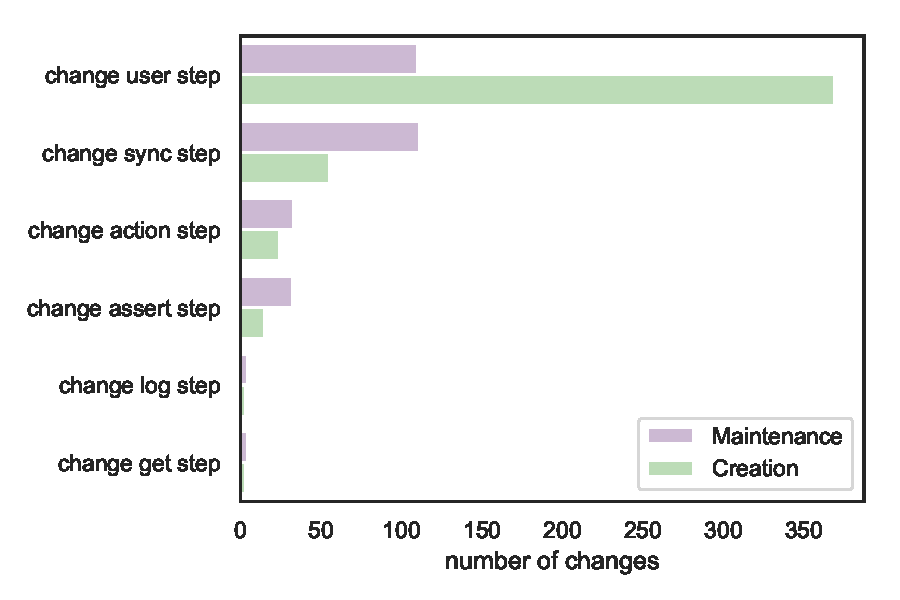
\includegraphics[width=0.7\columnwidth]{figures/evolution/changes_categories.pdf}
\caption{Total number of step changes per type}  
\label{fig:changes_steps}
\end{figure}

During \emph{Maintenance}, the main types of changes performed are the ``update step arguments'', the ``update step'', ``update documentation'' and ``insert user keyword''. After manually analyzing the changes to the arguments, we found two prevalent categories of commonly-changed arguments: arguments referring to \emph{synchronization} between the SUT and the KDT tests, e.g. wait 3 seconds and arguments referring to \emph{locators}, i.e., ways of locating elements in the GUI interface of the SUT. The arguments of the first category are typically used in the \emph{SYNC} category of Table \ref{keywords_categories}, and the latter at keywords of the \emph{ACTION} and \emph{ASSERTION} categories. Our results suggest that keywords belonging to these categories experience a high number of changes. Practitioners corroborate those results and motivate those results in RQ4.

\begin{figure}
\centering
\subfloat[Keyword Level \label{fig:boxplot_depth}]
    {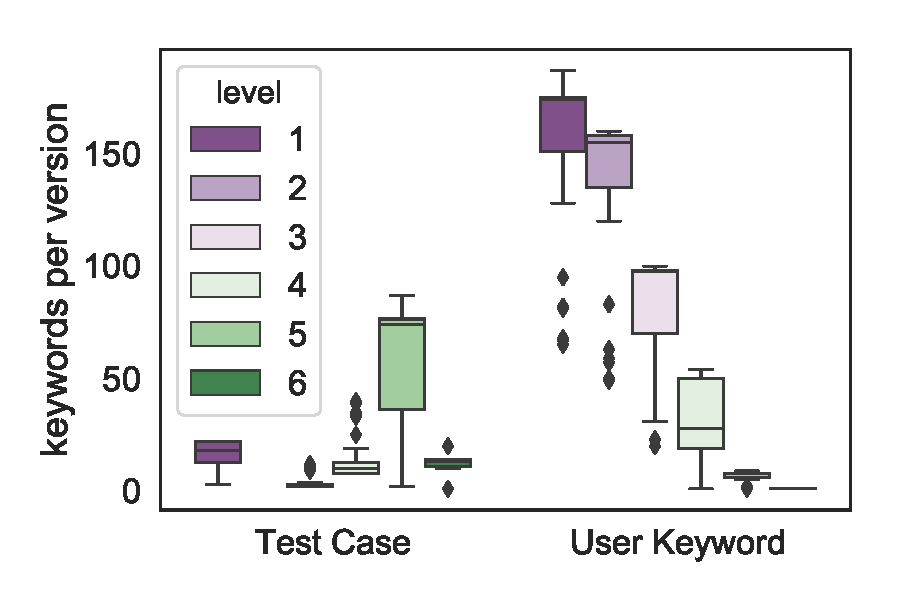
\includegraphics[width=0.7\textwidth]{figures/evolution/boxplot_depth.pdf}}
\subfloat[Keyword Connectivity\label{fig:boxplot_connectivity}]
    {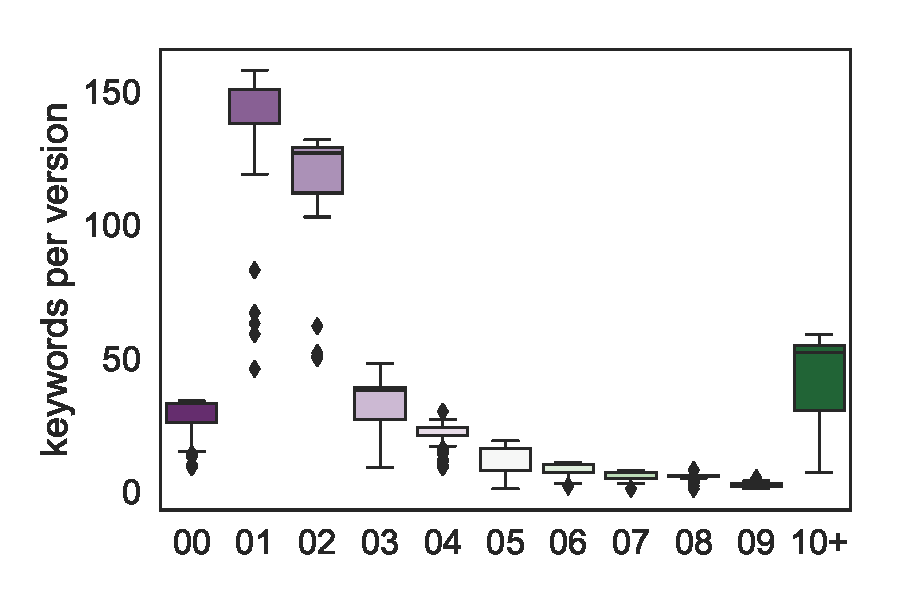
\includegraphics[width=0.7\textwidth]{figures/evolution/boxplot_connectivity.pdf}}
\subfloat[Connectivity per level category \label{fig:boxplot_depth_connectivity}]
    {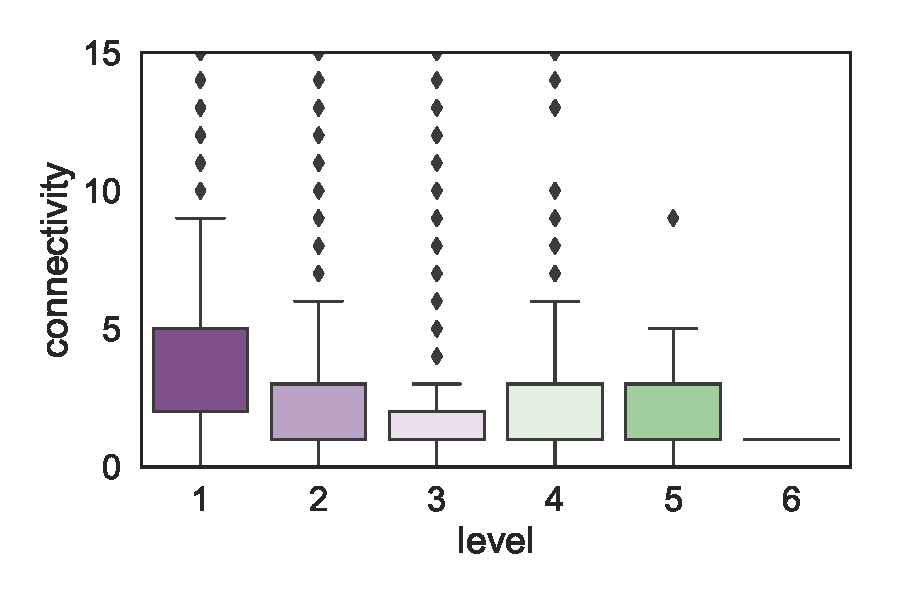
\includegraphics[width=0.7\textwidth]{figures/evolution/boxplot_depth_connectivity.pdf}}
\caption{Understanding KDT Test Suite Complexity}  
\label{fig:code_metrics}
\end{figure}

% susceptible to changes easily. The problem of defining \emph{locators} robust
% to changes has already been explored in the literature
% \cite{leotta_ICST_2015}.

Apart from ``update step arguments'', ``update step'' constitutes one of the most common change for both \emph{Creation} and \emph{Maintenance} periods. To further investigate the nature of these changes, Figure~\ref{fig:changes_steps} plots the number of changes (x-axis) against the category of the enclosing keywords (y-axis), as presented in Table~\ref{keywords_categories} with different colors for the periods studied.

As can be seen from the figure, \emph{change user steps} is by far the greatest activity during creation, we see that changes in \emph{synchronization steps} are equally important during maintenance. The interview conducted in RQ4 motivate that finding and explains it by the fact that many keywords are refactored during creation of new tests to become more generic so they can be reused. Another trend is that except for the \emph{user steps}, all other categories evolve more during maintenance. This is due to the same effect as mentioned earlier where changes in the application cause tests to break. \emph{user steps} are less affected by that effect since they are more abstract and thus less sensitive to trivial application evolution.

\subsection{RQ2: KDT Test Suite Complexity and Evolution}
\label{sec:evolution-results-rq2}

The results for RQ2 are split into two parts: first, results about the complexity of KDT test suites are reported; and, second, the way this complexity affects its evolution is presented.

\subsubsection{KDT test suite complexity}
\label{sec:kdt-test-suite}

To understand KDT test suite complexity, we calculate the \emph{keyword level} and \emph{connectivity} metrics, defined in Section~\ref{sec:evolution-protocol-definitions}. The first metric refers to the different ``abstraction levels'' (moving from pure technical to requirements expression) of the test suite and the second one, to the reusability among the keywords. Figures \ref{fig:boxplot_depth} and \ref{fig:boxplot_connectivity} present the corresponding results.

Figure~\ref{fig:boxplot_depth} depicts our results of the \emph{keyword level} for \emph{Test Cases} and \emph{User Keywords}, with the y-axis referring to the number of keywords per version. Recall that \emph{Test Cases} are the complete instantiation of a test - root node in the tree representation - and \emph{User Keywords} are user defined abstraction of the steps - intermediate nodes in the tree representation - (see also Section~\ref{kdt}). As can be seen from the figure, most \emph{Tests Cases} are relatively complex, with a level of 5, whereas most \emph{User Keywords} are simple (levels 1 to 2). This indicates that most user defined actions remain simple, in accordance with the philosophy of KDT.

Regarding the keyword reusability, Figure~\ref{fig:boxplot_connectivity} plots the number of keywords per version (y-axis) with the \emph{keyword connectivity} (x-axis). As can be seen, there is a high degree of reusability among \emph{User Keywords}. More precisely, only 20.34\% of the lines of code are used only once. Overall, the reused keywords amount to 51.56\% of the total lines of code of TestSuiteA. As we will see next, this reusability is key to the decreased cost of the KDT test suite maintenance.

Another interesting finding is the presence of dead test code, i.e., keywords not used anywhere in TestSuiteA; these keywords have a connectivity of 0 in Figure \ref{fig:boxplot_connectivity}. In total, 5.58\% of the keywords were not used, which amounts to 4.58\% of the test code base. When we presented our findings to the QA team, they were surprised and confirmed the existence of dead code, explaining that there is no tooling to support such analysis. Our tool solves this issue and it is planned to be integrated into the team's test code development processes.

To investigate whether keywords of a particular level tend to be more reused than others, Figure~\ref{fig:boxplot_depth_connectivity} plots the keyword connectivity among the different keyword levels. By examining the figure, it becomes clear that keywords levels exhibit relatively high connectivity, indicating that the reusability of keywords is not restricted to a particular level with the exception of level 1 showing a slightly higher connectivity.


% Manual analysis showed that this is due to the fact that different \emph{User
% Keywords} were created for different features of the software, therefore
% limiting reusability.

\subsubsection{KDT complexity and evolution}
\label{sec:kdt-compl-evol}

The second part of RQ2 refers to the evolution of KDT test suites and how their complexity affects it. To better understand the amount of changes performed during test code evolution, Figure~\ref{fig:churn} presents the test code churn (y-axis) over the eight-month period analyzed (x-axis), with a similar setup to Figure \ref{fig:project_evolution}.

The purple line in the figure denotes the average churn across TestSuiteA's evolution and the light purple, its variance represented here by the standard deviation. From the figure, it can be observed that during \emph{Creation}, the churn is 8.13\%, on average, whereas in the \emph{Maintenance} period, its value is 3.61\%. Overall, keywords are changed with a churn rate of 5.11\%. This number suggests that keywords are not entirely rewritten, but localized modifications are performed.

\begin{figure}
\centering
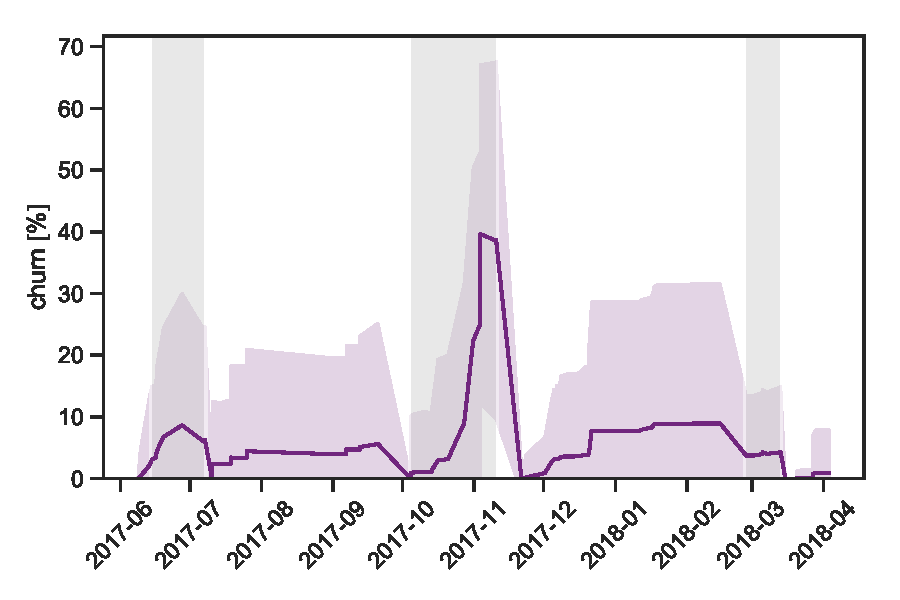
\includegraphics[width=0.7\columnwidth]{figures/evolution/time_series_churn.pdf}
\caption{KDT test code evolution: Churn over time}  
\label{fig:churn}
\end{figure}

To investigate further how the complexity of the KDT test code affects its evolution, Figure~\ref{fig:changes} plots the number of changes, for the whole period studied, against the keyword connectivity and level and Figure~\ref{fig:churn:analysis} plots the churn against the same metrics.

After examining Figure~\ref{fig:changes_connectivity}, it becomes clear that keyword reused one to three times are mostly changed. Keywords with higher connectivity do not change that often. Moreover, the figure shows that changes are performed on dead code (connectivity 0). This confirms that testers are unware of the fact that these keywords are never executed, generating easy to avoid maintenance. Regarding the results for changes and level, depicted in Figure~\ref{fig:changes_depth}, we can observe that the changes to \emph{Test Cases} do not follow a specific trend, whereas for the changes to the \emph{Users Keywords}, the lower level the keyword is, the more it is suceptible to be changed.

\begin{figure}
\centering
\subfloat[Connectivity \label{fig:changes_connectivity}]{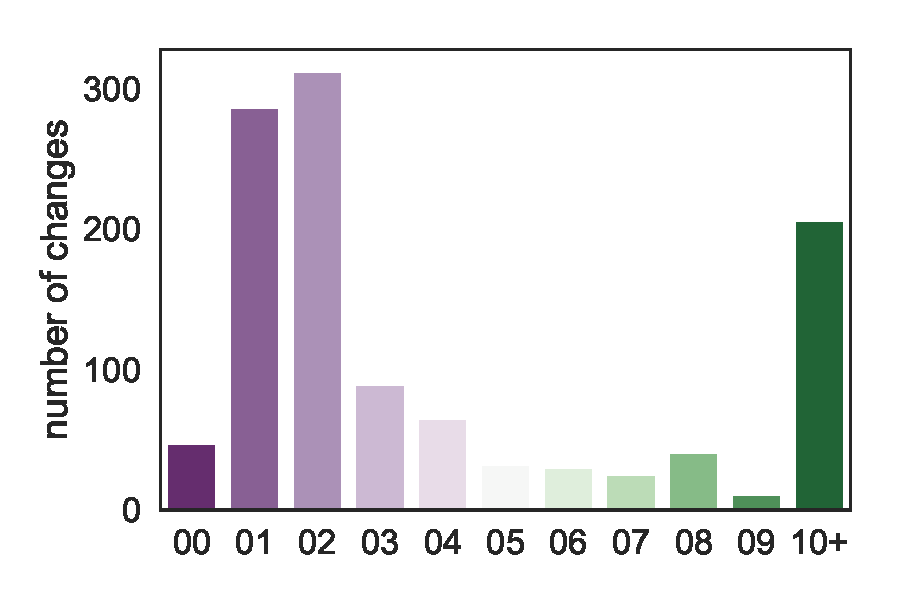
\includegraphics[width=0.7\textwidth]{figures/evolution/changes_connectivity_class_total.pdf}}
\subfloat[Level \label{fig:changes_depth}]{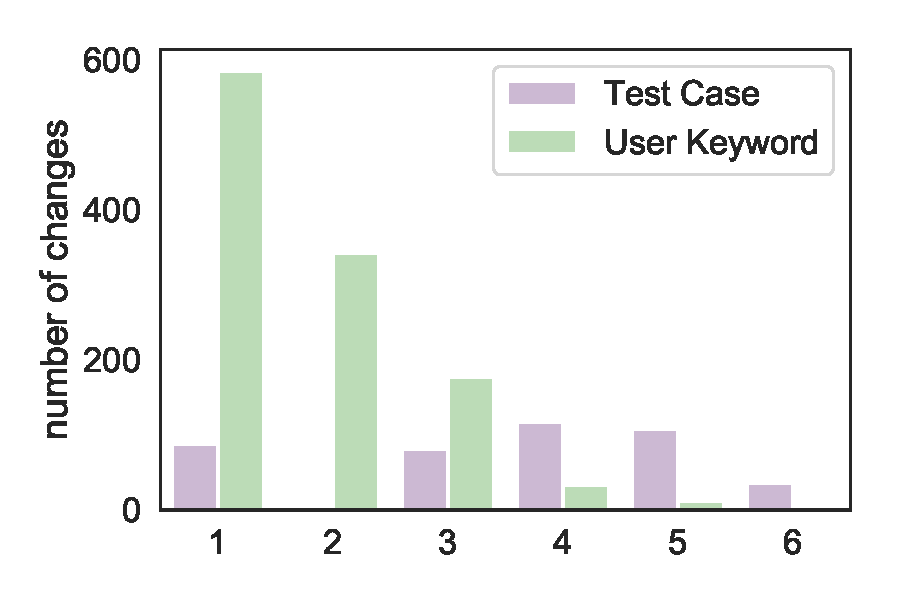
\includegraphics[width=0.7\textwidth]{figures/evolution/changes_depth_total.pdf}}
\caption{Changes distribution according to level and connectivity}  
\label{fig:changes}%\setlength{\tabcolsep}{5.1px} 
\end{figure}

\begin{figure}
\centering
\subfloat[Connectivity \label{fig:churn_connectivity}]{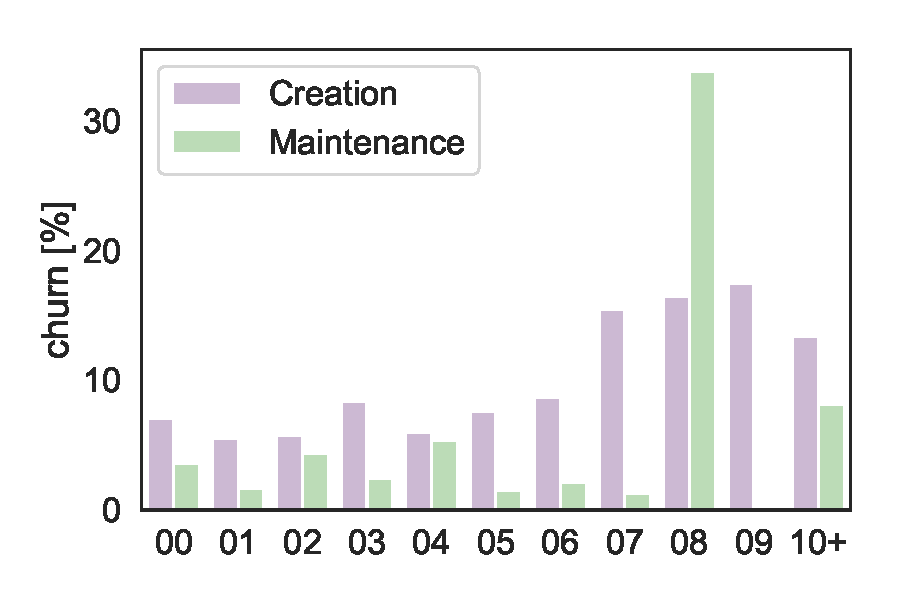
\includegraphics[width=0.7\textwidth]{figures/evolution/barplot_connectivity_class_churn.pdf}}
\subfloat[Level \label{fig:churn_depth}]{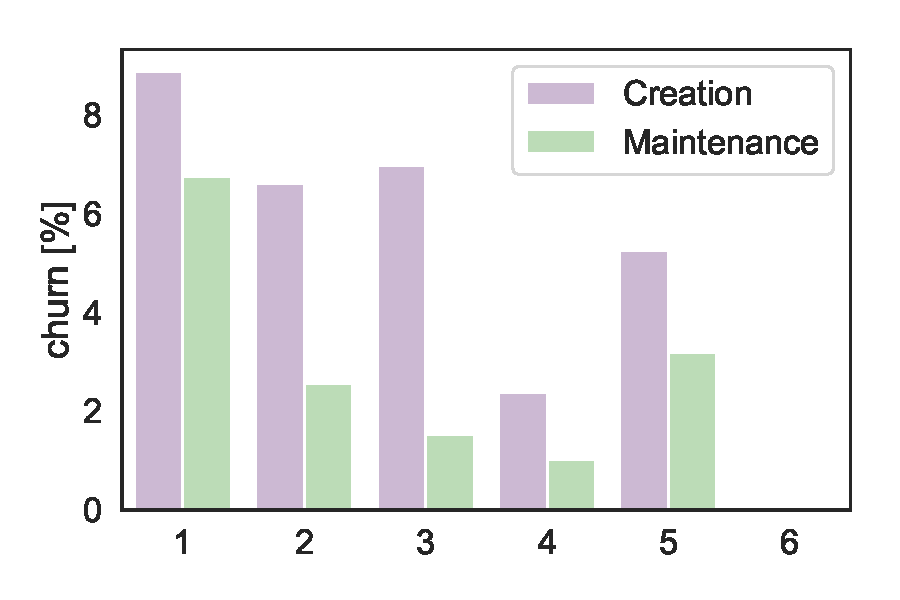
\includegraphics[width=0.7\textwidth]{figures/evolution/barplot_depth_churn.pdf}}
\caption{Churn distribution according to level and connectivity}  
\label{fig:churn:analysis}%\setlength{\tabcolsep}{5.1px} 
\end{figure}

Regarding our findings on the relation between churn rate and connectivity, depicted in Figure~\ref{fig:churn_connectivity} for the \emph{Creation} and \emph{Maintenance periods}, we can conclude that, during \emph{Creation}, keywords that are reused often, i.e. higher connectivity, exhibit approximately 50\%-60\% increased churn rate, whereas, during \emph{Maintenance} the opposite holds. Finally, regarding the results presented in Figure~\ref{fig:churn_depth} about churn and keyword level, we can see that, during \emph{Creation}, keywords with lower levels exhibit high churn values, whereas in \emph{Maintenance} this only holds for keywords of level 1. These results suggest that low level, highly reused keywords (basic action on the SUT), are evolving at a higher rate.

As we saw earlier, in TestSuiteA's evolution, keyword changed with a churn rate of 5.11\% but we also saw in the previous section that keywords are reused often. This raises the questions: How many changes have been saved due to the reusability of the keywords? To answer this question, we compare the the number of changes applied to TestSuiteA to the same suite without the keyword abstraction as explained in Section~\ref{sec:evolution-protocol-rq2}. We find that using KDT reduces the number of changes applied on TestSuiteA by 70.77\% during ``Creation'', by 72.69\% during ``Maintenance'' with an overall reduction during the entire period of 71.31\%. 

\subsection{RQ3: KDT, Test Clones and Evolution}
\label{sec:evolution-results-rq3}

In RQ3, we explore whether KDT test suites contain test clones and how these clones affect TestSuiteA's evolution. Table~\ref{table:co_evolution} presents the corresponding results. The table presents the total number of keywords that appear during the evolution of TestSuiteA (for all 129 versions) for each type of clone detected (first column -- Type I keyword clones, Type II and non-clones(``Others'')) and each type of evolution (second column). The types of evolution studied are the divided into three categories: keywords that are evolving strictly in the same way as others (``Co-evolution''), keywords that are evolving independently from others (``Evolution'') and keywords that do not evolve (``No change'').

We can observe several interesting findings from the table. First, we see that Type I and Type II clones comprise 30.2\% of the total amount keywords, indicating that almost one third of the test code written is duplicated. This finding highlights the fact that practitioners applying KDT will benefit from tools and techniques that can assist them in managing test clones.

Secondly, our results suggest that approximately 50\% of the Type I test clones evolve in the exact same way, indicating that the practitioners apply the same changes multiple times, wasting valuable effort. This is a high figure, especially when compared to the co-evolution of non-cloned keywords which is 4.9\%. Taking these results into consideration and the fact that almost 10\% of the keywords are evolving in the same way, it becomes obvious that automated refactoring techniques can reduce the maintenance effort of KDT test suite evolution.

\begin{table}
\caption{KDT Test Clones and Evolution}
\label{table:co_evolution}
\centering
\begin{tabular}{l|rrr|r}
  \toprule
         & \multicolumn{3}{c|}{Types of Evolution}                  \\
Keywords & Co-evolution &  Evolution &  No change &  Total          \\
\midrule
Type I  &          3526 &       3599 &        412 &   7537 (13.7\%) \\
Type II &           171 &       8462 &        491 &   9124 (16.5\%) \\  
Others  &          1888 &      33433 &       3184 &  38505 (69.8\%) \\
\midrule                                   
Total   &          5585 &      45494 &       4087 &  55166 (100\%)  \\ 
Percent &        10.1\% &     82.5\% &      7.4\% &    -            \\
\bottomrule
\end{tabular}
\end{table}

Finally, another interesting result exhibited in Table~\ref{table:co_evolution} concerns the overall evolution. We observe that only 7.4\% of the keywords are not evolving. This shows that during the TestSuiteA's evolution more than 90\% of the keywords are modified.

\subsection{RQ4: Benefits and challenges of KDT: The Practitioners' perspective}
\label{sec:evolution-results-rq4}

This research question pertains to the benefits and challenges of KDT as perceived by the practitioners. In the following, we present the main findings of our interviews grouped by the two main questions of our study:

\subsubsection{What are the benefits and challenges of adopting KDT?}

All interviewees agreed on two main benefits of KDT: the low learning curve and its simple syntax. Thanks to its syntax that is close to the natural language, new users can easily start being productive.  This syntax is also well-suited for communication purposes with teams that may have different backgrounds and expertise. The layered structure of keywords (i.e., the different keyword levels) plays an important role in facilitating this by hiding the technical details at the lower levels of the test suite and exhibiting the more business-oriented at the higher levels.

The main challenges encountered by the practitioners reside in their interaction with the SUT. Even a small evolution of the SUT can easily break the tests. Additionally, the testers discuss that finding the elements of the SUT that will be used in the tests is challenging, especially in applications where testability was not the primary concern.

\subsubsection{What kind of changes are performed on the test suite and why?}

The testers report two main reasons for the changes: SUT evolution and keyword adaptation.

Regarding the SUT evolution, the testers reported that as the SUT evolves, its components evolve as well which will cause the tests to adapt. The testers focus on two types of changes that are in according to our findings regarding RQ1 (cf. Section \ref{sec:evolution-results-rq1}): \emph{locators}, i.e., finding which GUI elements of the SUT should be used in the tests and \emph{synchronization} issues between the tests and the SUT.

Regarding keyword adaptation, the testers said that they create keywords in a ``best effort'' approach to cover the current needs. As new features of tests are developed, keywords are modified to become more generic. This fact explains the results illustrated in Figure~\ref{fig:changes_steps} where we observed many changes in \emph{user steps} during \emph{Creation}.

\section{Threats to Validity}

Threats to the external validity result from the generalization of our results outside the context of the study. Conducting the study with one industrial partner, the conclusions we draw may not be able to generalize to other companies using KDT. However, SubjectA is built using popular technologies, i.e., web frameworks and Java, which are wide-spread across the industry. Secondly and most important, this study is the first one, to the best of our knowledge, that analyzes the evolution of KDT test suites based on real-world data. Of course, this does not preclude the need for other studies to investigate further our results. Finally, another potential threat originates from the fact that we interviewed only 3 testers for RQ4.

Threats to the internal validity are due to the design of the study, potentially impacting our conclusions. The simple syntax of the test code allows for a robust model to be constructed. Our change algorithm presents some limitations: although phase 2 is based on the state of the art, it cannot detect \emph{Move} operations, resulting instead in two operations \emph{Delete} followed by an \emph{Insert}. This limitation might have influenced our results during the accounting of the number of changes. However, the rather low number of the \emph{delete step} operations (cf. Table \ref{table:total_changes}) indicates that this effect is marginal. Regarding the clone detection algorithm, as shown in \cite{Roy2009}, the rate of false-positives is known to be low for Type I and Type II clones.

Threat to construct validity result from the non suitability of the metrics used to evaluate the results. The main threat lies in the division of our work in two periods: ``Creation'' and ``Maintenance''. While empirical data motivated this separation, they lack of theoretical grounding. Further work on the test execution is needed to better motivate this decision.

\section{Conclusions}

Our results suggest that KDT test design is complex with several levels of abstraction and that this design favours reusability; more than 60\% of the keywords are reused which has the potential of reducing the changes needed during evolution up to 70\%.

Additionally, we find that keywords change with a relatively low rate (approximately 5\%) indicating that after a keyword's creation only fine-grained, localised changes are performed by the testers. Our results suggest that the most common changes to KDT tests are caused by \emph{synchronization} or element \emph{location} changes between the SUT and the test suite and to the \emph{assertions} of the tests. Our findings indicate that during evolution 90\% of the keywords evolve and that test clones exist in KDT test suites; approximately 30\% of the keywords are duplicated. Finally, we report on the practitioners' perception on the challenges and benefits of adopting KDT.